\documentclass[tikz,border=12pt]{standalone}
\usepackage[T1]{fontenc}
\usepackage{tgheros}
\usepackage{sfmath}
\usepackage{amsmath}
% % \usepackage{fontawesome5} (Removed for publication-grade academic typography) (Removed for publication-grade academic typography)
\usepackage{tikz}
\usetikzlibrary{arrows.meta,positioning,shapes.geometric,fit,backgrounds,calc}
\usepackage{xcolor}

\renewcommand{\familydefault}{\sfdefault}

% Semantic Palette from visual-system.md
\definecolor{navy}{HTML}{1B2A4A}
\definecolor{navylight}{HTML}{E8EDF6}
\definecolor{teal}{HTML}{168F84}
\definecolor{teallight}{HTML}{E4F6F3}
\definecolor{amber}{HTML}{C98218}
\definecolor{amberlight}{HTML}{FFF3DC}
\definecolor{coral}{HTML}{BD4F2F}
\definecolor{corallight}{HTML}{FAE9E2}
\definecolor{violet}{HTML}{6550A8}
\definecolor{violetlight}{HTML}{F0ECFA}
\definecolor{slate}{HTML}{687386}
\definecolor{slatelight}{HTML}{F4F6F7}
\definecolor{cardborder}{HTML}{CBD5E1}

\begin{document}
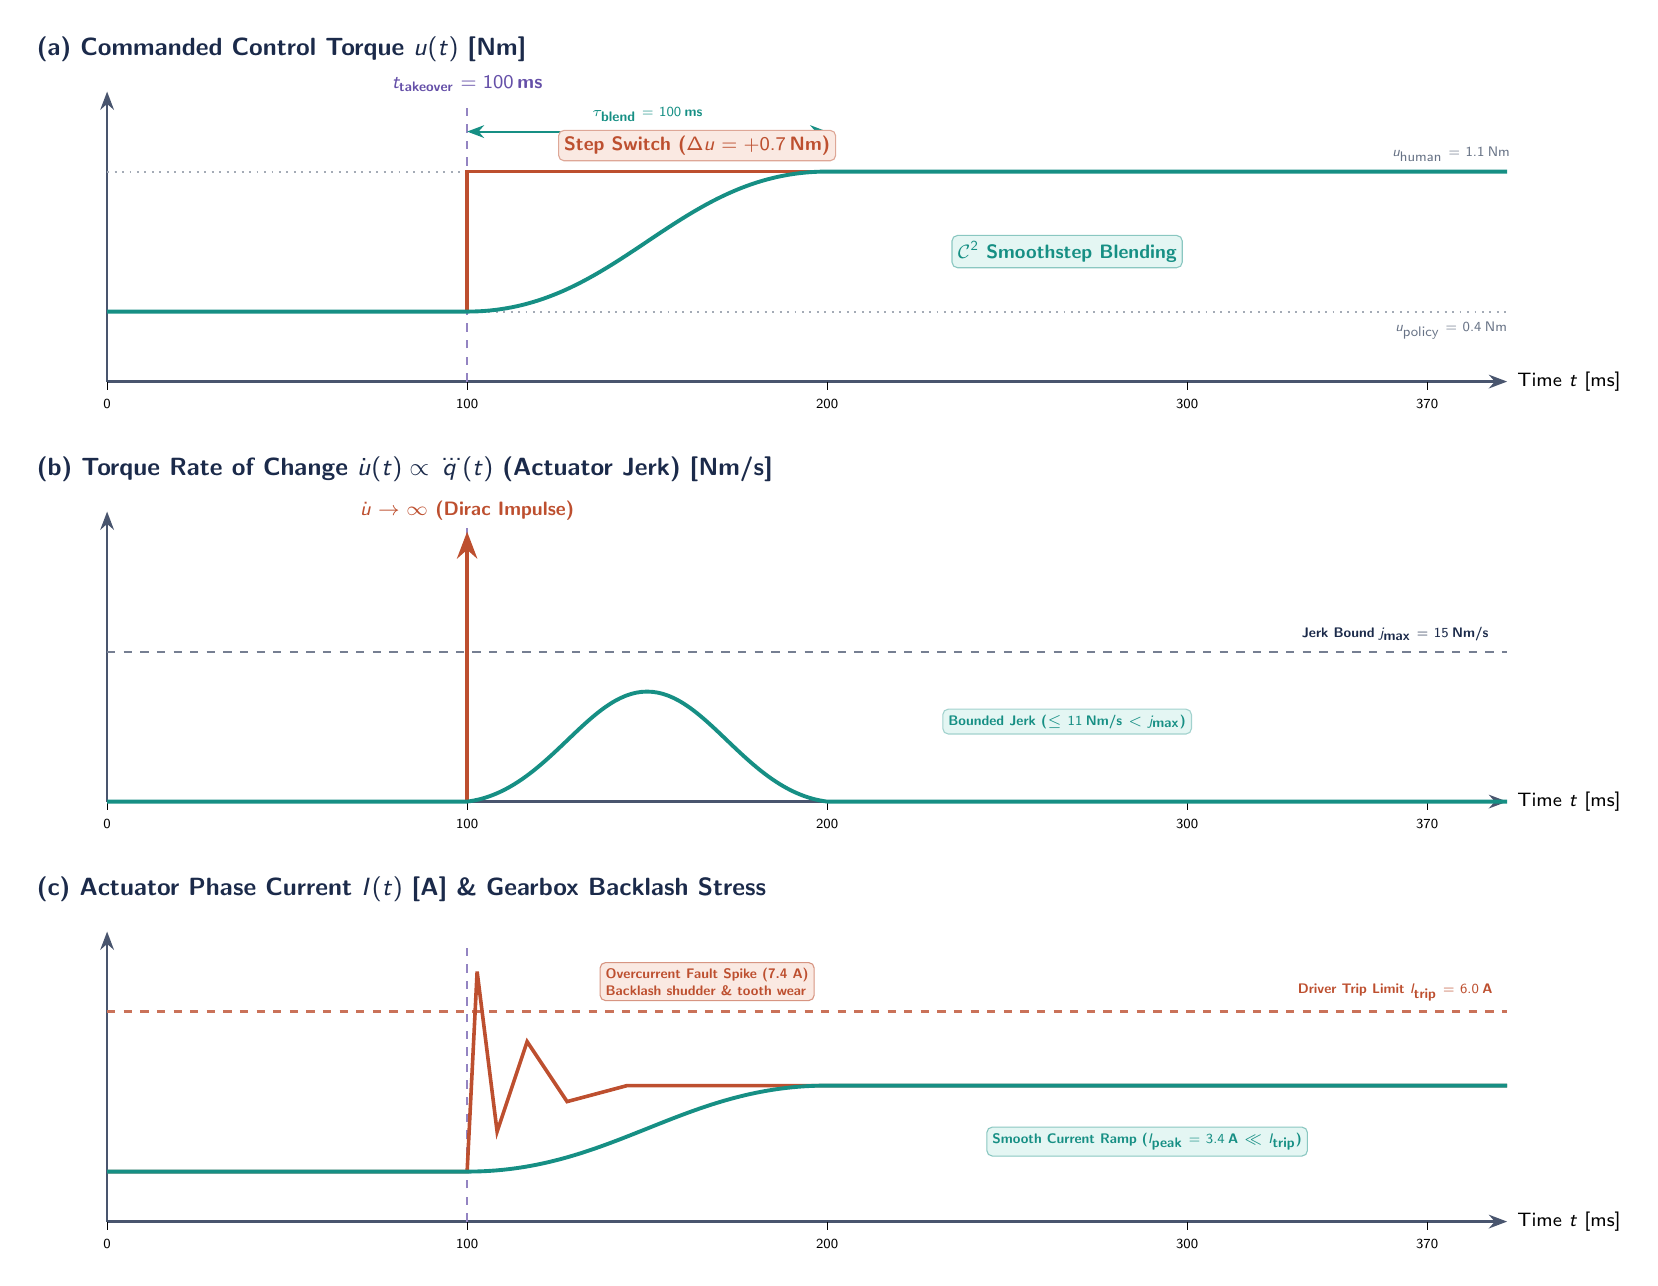
\begin{tikzpicture}[
  font=\sffamily,
  >=Stealth,
  axisline/.style={->, line width=0.8pt, draw=navy!80},
  gridline/.style={draw=slate!25, line width=0.4pt, dashed},
  stepcurve/.style={draw=coral, line width=1.3pt},
  blendcurve/.style={draw=teal, line width=1.4pt},
  refcurve/.style={draw=slate!60, line width=0.7pt, dotted},
  badgenode/.style={font=\sffamily\scriptsize\bfseries, fill=white, draw=cardborder, rounded corners=2pt, inner sep=2pt}
]

  % =========================================================================
  % PANEL 1: COMMANDED TORQUE / TRAJECTORY u(t)
  % =========================================================================
  \coordinate (p1_origin) at (0, 0);
  
  \node[anchor=south west, font=\sffamily\small\bfseries, text=navy] at ($(p1_origin)+(-0.4in, 1.55in)$) {
     (a) Commanded Control Torque $u(t)$ [Nm]
  };

  % Axes
  \draw[axisline] (p1_origin) -- ++(7.0in, 0) node[right, font=\sffamily\scriptsize] {Time $t$ [ms]};
  \draw[axisline] (p1_origin) -- ++(0, 1.45in);

  % Vertical Takeover Line at t=100ms
  \coordinate (t_takeover_1) at ($(p1_origin)+(1.8in, 0)$);
  \draw[dashed, line width=0.8pt, draw=violet!70] (t_takeover_1) -- ++(0, 1.4in)
    node[pos=1.0, above, font=\sffamily\scriptsize\bfseries, text=violet] {$t_{\text{takeover}} = 100\,\text{ms}$};

  % Blend window span
  \coordinate (t_blend_end_1) at ($(t_takeover_1)+(1.8in, 0)$);
  \draw[<->, line width=0.7pt, draw=teal] ($(t_takeover_1)+(0, 1.25in)$) -- ($(t_blend_end_1)+(0, 1.25in)$)
    node[pos=0.5, above, font=\sffamily\tiny\bfseries, text=teal] {$\tau_{\text{blend}} = 100\,\text{ms}$};

  % Ticks
  \foreach \x/\label in {0/0, 1.8/100, 3.6/200, 5.4/300, 6.6/370} {
    \draw ($(p1_origin)+(\x in, 0)$) -- ++(0, -3pt) node[below, font=\sffamily\tiny] {\label};
  }

  % Reference Autonomous & Human levels
  \draw[refcurve] ($(p1_origin)+(0, 0.35in)$) -- ($(p1_origin)+(7.0in, 0.35in)$)
    node[pos=0.96, below, font=\sffamily\tiny, text=slate] {$u_{\text{policy}} = 0.4\,\text{Nm}$};
  \draw[refcurve] ($(p1_origin)+(0, 1.05in)$) -- ($(p1_origin)+(7.0in, 1.05in)$)
    node[pos=0.96, above, font=\sffamily\tiny, text=slate] {$u_{\text{human}} = 1.1\,\text{Nm}$};

  % Step Takeover Curve (Coral)
  \draw[stepcurve] ($(p1_origin)+(0, 0.35in)$) -- ($(p1_origin)+(1.8in, 0.35in)$) 
    -- ($(p1_origin)+(1.8in, 1.05in)$) -- ($(p1_origin)+(7.0in, 1.05in)$);
  \node[font=\sffamily\scriptsize\bfseries, text=coral, fill=corallight, draw=coral!50, rounded corners=2pt, inner sep=2pt] 
    at ($(p1_origin)+(2.95in, 1.18in)$) { Step Switch ($\Delta u = +0.7\,\text{Nm}$)};

  % Bumpless Blended Curve (Teal S-Curve)
  \draw[blendcurve] ($(p1_origin)+(0, 0.35in)$) -- ($(p1_origin)+(1.8in, 0.35in)$)
    to[out=0, in=180] ($(p1_origin)+(3.6in, 1.05in)$) -- ($(p1_origin)+(7.0in, 1.05in)$);
  \node[font=\sffamily\scriptsize\bfseries, text=teal, fill=teallight, draw=teal!50, rounded corners=2pt, inner sep=2pt] 
    at ($(p1_origin)+(4.8in, 0.65in)$) { $\mathcal{C}^2$ Smoothstep Blending};

  % =========================================================================
  % PANEL 2: TORQUE DERIVATIVE / MOTOR JERK \dot{u}(t)
  % =========================================================================
  \coordinate (p2_origin) at (0, -2.1in);
  
  \node[anchor=south west, font=\sffamily\small\bfseries, text=navy] at ($(p2_origin)+(-0.4in, 1.55in)$) {
     (b) Torque Rate of Change $\dot{u}(t) \propto \dddot{q}(t)$ (Actuator Jerk) [Nm/s]
  };

  % Axes
  \draw[axisline] (p2_origin) -- ++(7.0in, 0) node[right, font=\sffamily\scriptsize] {Time $t$ [ms]};
  \draw[axisline] (p2_origin) -- ++(0, 1.45in);

  % Ticks
  \foreach \x/\label in {0/0, 1.8/100, 3.6/200, 5.4/300, 6.6/370} {
    \draw ($(p2_origin)+(\x in, 0)$) -- ++(0, -3pt) node[below, font=\sffamily\tiny] {\label};
  }

  % Vertical Takeover Line at t=100ms
  \coordinate (t_takeover_2) at ($(p2_origin)+(1.8in, 0)$);
  \draw[dashed, line width=0.8pt, draw=violet!70] (t_takeover_2) -- ++(0, 1.4in);

  % Jerk limit threshold
  \draw[dashed, line width=0.7pt, draw=navy!60] ($(p2_origin)+(0, 0.75in)$) -- ($(p2_origin)+(7.0in, 0.75in)$)
    node[pos=0.92, above, font=\sffamily\tiny\bfseries, text=navy] {Jerk Bound $j_{\text{max}} = 15\,\text{Nm/s}$};

  % Step Takeover Jerk Spike (Coral impulse)
  \draw[stepcurve, ->, >=Stealth, line width=1.5pt] (t_takeover_2) -- ++(0, 1.35in)
    node[above, font=\sffamily\scriptsize\bfseries, text=coral] {$\dot{u} \to \infty$ (Dirac Impulse)};

  % Bumpless Jerk Profile (Teal Smooth Bell Curve)
  \draw[blendcurve] ($(p2_origin)+(0, 0)$) -- ($(p2_origin)+(1.8in, 0)$)
    .. controls ($(p2_origin)+(2.2in, 0.05in)$) and ($(p2_origin)+(2.4in, 0.55in)$) .. ($(p2_origin)+(2.7in, 0.55in)$)
    .. controls ($(p2_origin)+(3.0in, 0.55in)$) and ($(p2_origin)+(3.2in, 0.05in)$) .. ($(p2_origin)+(3.6in, 0)$)
    -- ($(p2_origin)+(7.0in, 0)$);

  \node[font=\sffamily\tiny\bfseries, text=teal, fill=teallight, draw=teal!40, rounded corners=2pt, inner sep=2pt]
    at ($(p2_origin)+(4.8in, 0.40in)$) {Bounded Jerk ($\le 11\,\text{Nm/s} < j_{\text{max}}$)};

  % =========================================================================
  % PANEL 3: MOTOR PHASE CURRENT I(t) & MECHANICAL IMPACT
  % =========================================================================
  \coordinate (p3_origin) at (0, -4.2in);
  
  \node[anchor=south west, font=\sffamily\small\bfseries, text=navy] at ($(p3_origin)+(-0.4in, 1.55in)$) {
     (c) Actuator Phase Current $I(t)$ [A] \& Gearbox Backlash Stress
  };

  % Axes
  \draw[axisline] (p3_origin) -- ++(7.0in, 0) node[right, font=\sffamily\scriptsize] {Time $t$ [ms]};
  \draw[axisline] (p3_origin) -- ++(0, 1.45in);

  % Ticks
  \foreach \x/\label in {0/0, 1.8/100, 3.6/200, 5.4/300, 6.6/370} {
    \draw ($(p3_origin)+(\x in, 0)$) -- ++(0, -3pt) node[below, font=\sffamily\tiny] {\label};
  }

  % Overcurrent Trip Threshold
  \draw[dashed, line width=0.8pt, draw=coral!80] ($(p3_origin)+(0, 1.05in)$) -- ($(p3_origin)+(7.0in, 1.05in)$)
    node[pos=0.92, above, font=\sffamily\tiny\bfseries, text=coral] {Driver Trip Limit $I_{\text{trip}} = 6.0\,\text{A}$};

  % Vertical Takeover Line
  \coordinate (t_takeover_3) at ($(p3_origin)+(1.8in, 0)$);
  \draw[dashed, line width=0.8pt, draw=violet!70] (t_takeover_3) -- ++(0, 1.4in);

  % Step Takeover Current (Severe Inrush Spike + High Frequency Ringing)
  \draw[stepcurve] ($(p3_origin)+(0, 0.25in)$) -- ($(p3_origin)+(1.8in, 0.25in)$)
    -- ($(p3_origin)+(1.85in, 1.25in)$) 
    -- ($(p3_origin)+(1.95in, 0.45in)$)
    -- ($(p3_origin)+(2.10in, 0.90in)$)
    -- ($(p3_origin)+(2.30in, 0.60in)$)
    -- ($(p3_origin)+(2.60in, 0.68in)$)
    -- ($(p3_origin)+(7.0in, 0.68in)$);

  \node[font=\sffamily\tiny\bfseries, text=coral, fill=corallight, draw=coral!60, rounded corners=2pt, inner sep=2pt, align=left]
    at ($(p3_origin)+(3.0in, 1.20in)$) {\textbf{Overcurrent Fault Spike (7.4 A)}\\Backlash shudder \& tooth wear};

  % Bumpless Blended Current (Smooth ramp from 0.25in to 0.68in)
  \draw[blendcurve] ($(p3_origin)+(0, 0.25in)$) -- ($(p3_origin)+(1.8in, 0.25in)$)
    to[out=0, in=180] ($(p3_origin)+(3.6in, 0.68in)$)
    -- ($(p3_origin)+(7.0in, 0.68in)$);

  \node[font=\sffamily\tiny\bfseries, text=teal, fill=teallight, draw=teal!50, rounded corners=2pt, inner sep=2pt]
    at ($(p3_origin)+(5.2in, 0.40in)$) {\textbf{Smooth Current Ramp} ($I_{\text{peak}} = 3.4\,\text{A} \ll I_{\text{trip}}$)};

\end{tikzpicture}
\end{document}
